\chapter{METHODOLOGY}

\begin{figure}[ht]
    \centering
    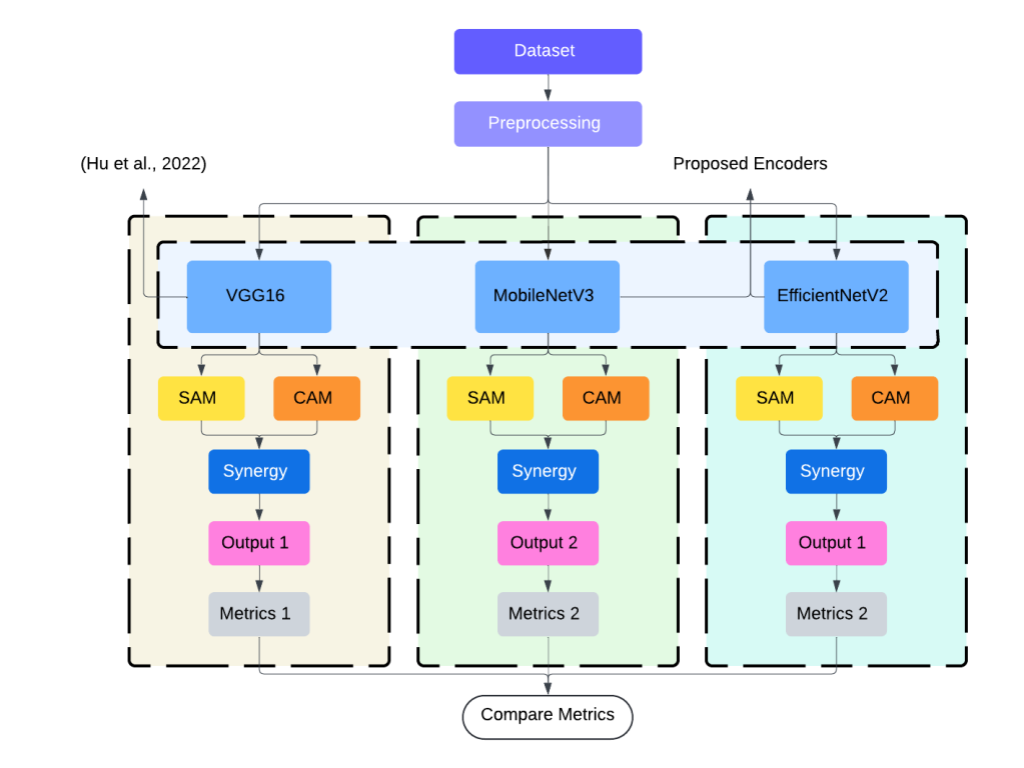
\includegraphics[width=0.9\textwidth]{figures/asnet-architecture/placeholder_conceptual_framework.png} 
    \caption[Conceptual Framework of the Study]{Conceptual framework illustrating the research methodology. The BraTS 2023-GLI (Task 1) dataset undergoes preprocessing before being fed into different AS-Net variants. The baseline uses the VGG16 encoder (Hu et al., 2022), while the proposed variants use MobileNetV3 and EfficientNetV2 encoders. Each variant employs the core AS-Net modules (SAM, CAM, Synergy) to produce segmentation outputs. Performance metrics are calculated for each variant and then compared to evaluate the effectiveness and efficiency of the different encoders.}
    \label{fig:conceptual_framework}
\end{figure}

Figure \ref{fig:conceptual_framework} outlines the conceptual framework guiding this research. The process begins with the BraTS 2023-GLI (Task 1) dataset, which undergoes a standardized preprocessing pipeline (converting NIfTI to HDF5 slices). The preprocessed data serves as input to multiple parallel streams, each representing an implementation of the Attention Synergy Network (AS-Net). One stream utilizes the original VGG16 encoder as a baseline, reflecting the approach by \textcite{hu2022net}. The other streams employ the proposed lightweight encoders: MobileNetV3 (Large and Small) and EfficientNetV2 (B0 and B1). Regardless of the encoder, each AS-Net variant incorporates the core Spatial Attention Module (SAM), Channel Attention Module (CAM), and Synergy module within its decoder structure to generate segmentation outputs. Performance metrics (segmentation accuracy and computational efficiency) are computed for each model variant based on these outputs. Finally, these metrics are systematically compared to assess the relative advantages and disadvantages of the different encoder backbones within the AS-Net framework for MRI brain tumor segmentation.

\section{Dataset and Preprocessing}

The study utilized the BraTS 2023-GLI (Task 1) (Brain Tumor Segmentation) challenge training dataset, which had been pre-processed from NIfTI format into a collection of HDF5 (H5) files, each representing a single 2D axial slice. This format facilitated efficient data loading and processing.

\subsection{Data Source and Structure}
The original BraTS 2023-GLI dataset provides multi-modal 3D MRI scans (T1, T1ce, T2, FLAIR) and corresponding ground truth segmentation masks. The preprocessing script converted these into H5 files where each file contained:
\begin{itemize}
    \item \texttt{image}: A numpy array (e.g., 240x240x4) containing pixel data for the four standard MRI modalities for a single axial slice.
    \item \texttt{mask}: A numpy array (e.g., 240x240x3) representing the expert-annotated ground truth segmentation masks for tumor sub-regions (NCR/NET, ED, ET) for that slice.
\end{itemize}
A metadata CSV file provided the mapping between patient identifiers, slice indices, and H5 file paths.

\subsection{Data Loading and Preprocessing Pipeline}
A custom data loading and preprocessing pipeline was implemented using TensorFlow's \texttt{tf.data} API for efficiency and integration with distributed training strategies. This pipeline performed the following steps for each H5 file:

\begin{enumerate}
    \item \textbf{File Path Handling:} Read file paths from the metadata CSV, filtering for existing files.
    \item \textbf{Data Splitting:} Randomly shuffled the dataset (using a fixed seed for reproducibility) and split it into training (80\%), validation (10\%), and test (10\%) sets based on the file list.
    \item \textbf{H5 File Parsing:} Loaded the \texttt{image} and \texttt{mask} arrays from each H5 file.
    \item \textbf{Modality Selection:} Selected the T1ce (index 1) and FLAIR (index 3) modalities from the 4-channel \texttt{image} array.
    \item \textbf{RGB Channel Mapping:} Mapped the two selected modalities ([T1ce, FLAIR]) to a 3-channel format suitable for the pre-trained encoders using indices [0, 1, 0], resulting in an input representation of [T1ce, FLAIR, T1ce].
    \item \textbf{Normalization:} Applied Z-score normalization independently to each selected input channel (T1ce and FLAIR) *before* the RGB mapping. The mean and standard deviation were calculated on a per-slice, per-channel basis.
    \item \textbf{Binary Mask Creation:} Converted the multi-channel ground truth \texttt{mask} into a single-channel binary mask. Any voxel labeled as part of the tumor (NCR/NET, ED, or ET) was assigned a value of 1, while all other voxels (background) were assigned 0. This binary mask served as the target for the segmentation loss function.
    \item \textbf{Multi-Class Mask Preparation:} Created a multi-class mask representation for visualization purposes, mapping NCR/NET to 1, ED to 2, and ET to 4 (overwriting in case of overlap), with background as 0.
    \item \textbf{Resizing:} Resized the 3-channel input image and the single-channel binary mask to the specific target dimensions required by each encoder architecture using \texttt{tf.image.resize}. Bilinear interpolation was used for the images, and nearest-neighbor interpolation was used for the masks to preserve label integrity. The target sizes were:
        \begin{itemize}
            \item VGG16: 224x224
            \item MobileNetV3-Large, MobileNetV3-Small, EfficientNetV2-B0: 224x224
            \item EfficientNetV2-B1: 240x240
        \end{itemize}
    \item \textbf{Visualization Data Preparation:} Resized the selected reference modality (FLAIR) and the multi-class mask to the target dimensions for use in generating qualitative results, normalizing the reference image to [0, 1].
    \item \textbf{Batching and Prefetching:} Grouped the processed samples into batches according to the global batch size and used \texttt{tf.data.AUTOTUNE} for prefetching to optimize GPU utilization.
\end{enumerate}
The final output structure yielded by the data pipeline for each batch consisted of a tuple: \texttt{model\_input\_image}, \texttt{binary\_ground\_truth\_mask}, \texttt{reference\_display\_image}, \texttt{multi\_class\_display\_mask}. Only the first two elements were used during model training and quantitative evaluation.

\section{AS-Net Architecture Adaptation}

The study adapted the AS-Net architecture by combining its core attention and synergy modules with different encoder backbones.

\subsection{Encoder Networks}
Five pre-trained encoder networks were integrated into the AS-Net framework, leveraging weights learned from the ImageNet dataset:

\begin{enumerate}
    \item \textbf{VGG16:} Used as the baseline encoder, adapted from the original AS-Net paper \parencite{hu2022net}. Input size: 224x224x3.
    \item \textbf{MobileNetV3-Large:} A high-performance lightweight encoder. Input size: 224x224x3.
    \item \textbf{MobileNetV3-Small:} An efficiency-focused lightweight encoder. Input size: 224x224x3.
    \item \textbf{EfficientNetV2-B0:} The smallest variant of the EfficientNetV2 family. Input size: 224x224x3.
    \item \textbf{EfficientNetV2-B1:} A slightly larger EfficientNetV2 variant. Input size: 240x240x3.
\end{enumerate}

For MobileNetV3 and EfficientNetV2, their respective built-in \texttt{preprocess\_input} functions were applied as the first step within the model definition to scale the input pixel values appropriately. For VGG16, the Z-score normalization applied during data preprocessing served as the input normalization.

\textbf{Fine-tuning Strategy:} A transfer learning approach with fine-tuning was employed. The initial convolutional blocks of each pre-trained encoder were frozen (weights were not updated during training), while the later blocks were unfrozen and allowed to train. The specific layers marking the transition from frozen to trainable were chosen based on common practices for transfer learning with these architectures (e.g., starting from 'block4' for VGG16, 'expanded\_conv\_6' for MobileNetV3-Large, 'block4' for EfficientNetV2 variants). This strategy aimed to retain general features learned from ImageNet while adapting the deeper layers to the specifics of MRI brain tumor segmentation.

\subsection{Core AS-Net Modules (SAM, CAM, Synergy)}
The core components of the AS-Net decoder were used consistently across all encoder variants:

\begin{itemize}
    \item \textbf{Spatial Attention Module (SAM):} As illustrated in Figure \ref{fig:sam_module}, SAM processes input features through parallel convolutional pathways. One pathway generates spatial attention maps using pooling and upsampling to capture multi-scale spatial context, highlighting salient regions (likely tumor areas). These maps weight the features from the other pathway, effectively focusing computation on relevant spatial locations.
    \item \textbf{Channel Attention Module (CAM):} As shown in Figure \ref{fig:cam_module}, CAM focuses on inter-channel relationships. It uses global average pooling to squeeze spatial information, followed by a small multi-layer perceptron (MLP) operating on channel descriptors to generate channel-wise attention weights. These weights rescale the input feature channels, emphasizing informative features and suppressing less useful ones.
    \item \textbf{Synergy Module:} This module integrates the outputs from the parallel SAM and CAM branches. It computes a weighted sum of the SAM and CAM feature maps using learnable scalar parameters ($\alpha$ and $\beta$, initialized to 0.5 and trained alongside the network). This adaptive fusion is followed by a 1x1 convolution and Batch Normalization to refine the combined features before passing them to the next decoder stage.
\end{itemize}

A custom \texttt{ResizeToMatchLayer} was introduced and utilized specifically in the EfficientNetV2 decoder. This layer addresses potential minor discrepancies in spatial dimensions between upsampled features and skip connection features that can arise due to padding or striding differences in the EfficientNetV2 architecture, ensuring compatible shapes for the concatenation operation in the decoder.

% SAM Figure
\begin{figure}[ht]
    \centering
	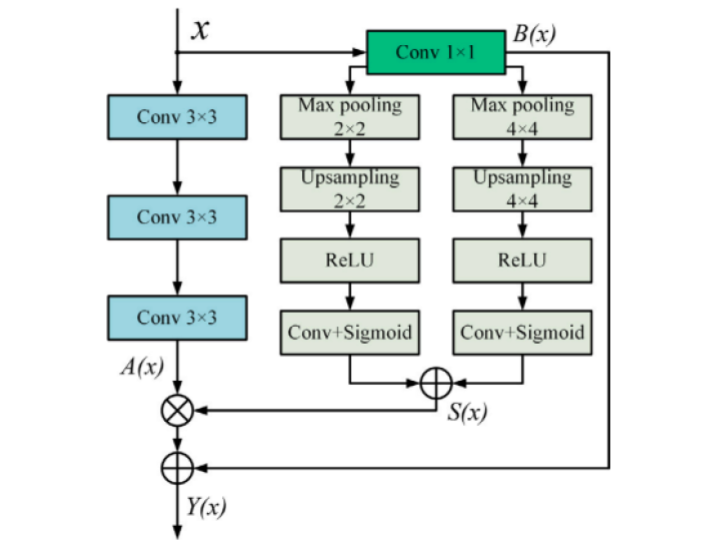
\includegraphics[width=0.85\textwidth]{figures/asnet-architecture/placeholder_sam_diagram.png}
	\caption[Spatial Attention Module (SAM)]{Diagram of the Spatial Attention Module (SAM) used in the AS-Net decoder.}
	\label{fig:sam_module}
\end{figure}

% CAM Figure
\begin{figure}[ht]
    \centering
	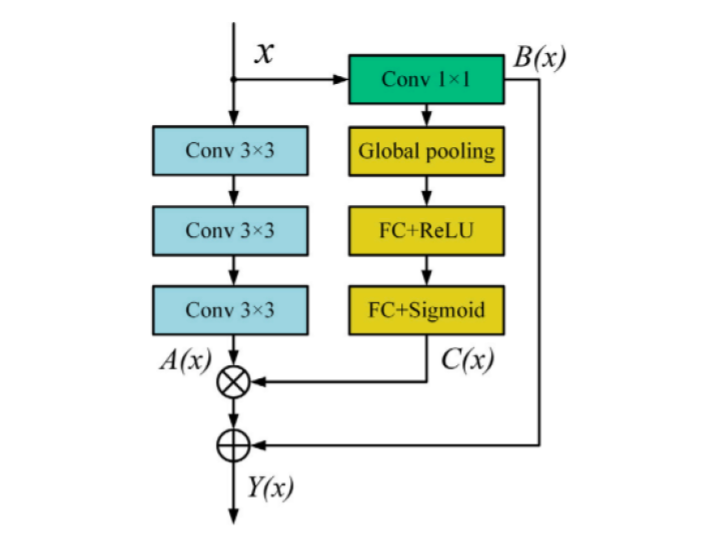
\includegraphics[width=0.85\textwidth]{figures/asnet-architecture/placeholder_cam_diagram.png}
	\caption[Channel Attention Module (CAM)]{Diagram of the Channel Attention Module (CAM) used in the AS-Net decoder.}
	\label{fig:cam_module}
\end{figure}

\subsection{Decoder Structure}
The decoder followed a standard U-Net-like symmetric structure, designed to progressively upsample features while integrating high-resolution spatial information from the encoder via skip connections. At each decoder stage:
\begin{enumerate}
    \item The feature map from the preceding decoder stage was upsampled by a factor of 2 using bilinear interpolation (\texttt{UpSampling2D}).
    \item The upsampled feature map was concatenated with the corresponding feature map extracted from the encoder backbone at the same spatial resolution (skip connection).
    \item The concatenated feature map was fed into parallel SAM and CAM modules.
    \item The outputs of the SAM and CAM modules were fused using the Synergy module.
    \item The output of the Synergy module was passed to the next decoder stage.
\end{enumerate}
This process was repeated across multiple stages (typically 4 stages, corresponding to the skip connections used). After the final upsampling stage, which restored the feature map to the original input resolution, a 1x1 convolutional layer with a sigmoid activation function was applied. This final layer produced a single-channel output map representing the pixel-wise probability of belonging to the tumor class (values between 0 and 1).

Figure \ref{fig:asnet_vgg16_arch}, Figure \ref{fig:asnet_mobilenet_arch}, and Figure \ref{fig:asnet_efficientnet_arch} provide high-level illustrations of the AS-Net architecture incorporating the different encoder types.

% Architecture Figures
\begin{figure}[!htb]
    \centering
	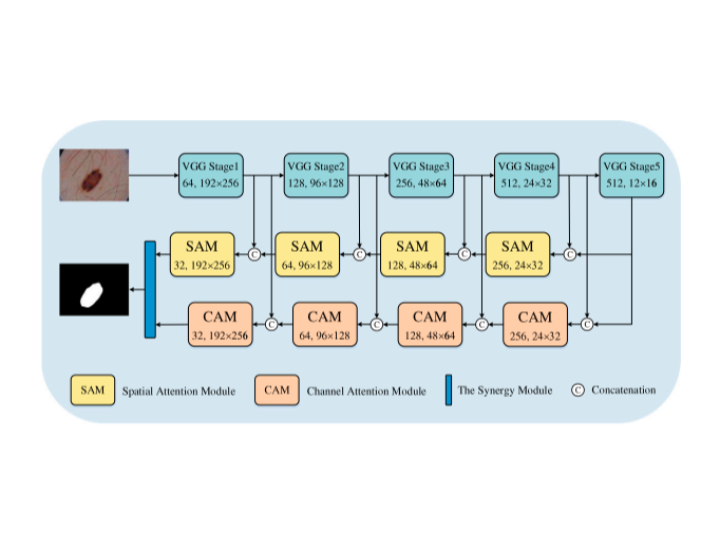
\includegraphics[width=0.85\textwidth]{figures/asnet-encoders/placeholder_asnet_vgg16.png}
	\caption[AS-Net Architecture with VGG16 Encoder]{High-level architecture of AS-Net using the VGG16 encoder backbone.}
	\label{fig:asnet_vgg16_arch}
\end{figure}

\begin{figure}[!htb]
    \centering
    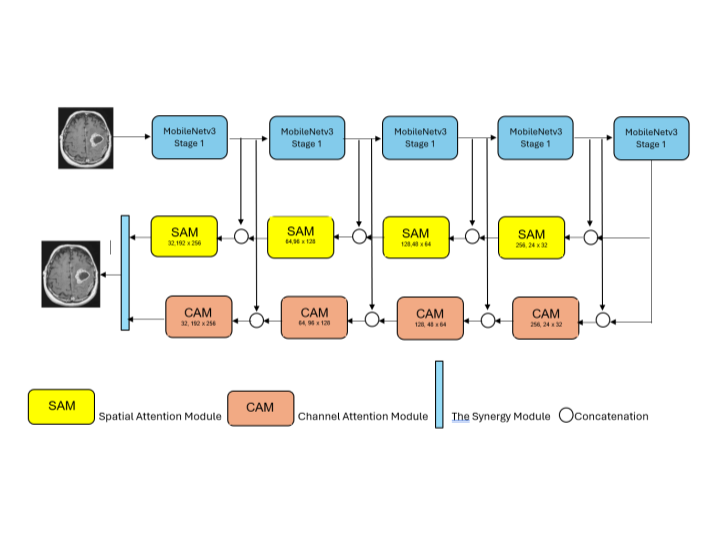
\includegraphics[width=0.85\textwidth]{figures/asnet-encoders/placeholder_asnet_mobilenet.png}
    \caption[AS-Net Architecture with MobileNetV3 Encoder]{High-level architecture of AS-Net using MobileNetV3 (Large/Small) encoder backbones.}
    \label{fig:asnet_mobilenet_arch}
\end{figure}

\begin{figure}[!htb]
    \centering
    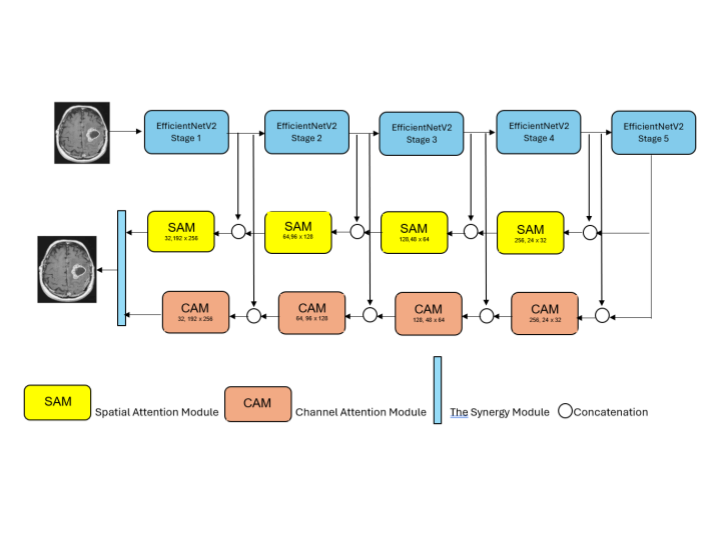
\includegraphics[width=0.85\textwidth]{figures/asnet-encoders/placeholder_asnet_efficientnet.png}
    \caption[AS-Net Architecture with EfficientNetV2 Encoder]{High-level architecture of AS-Net using EfficientNetV2 (B0/B1) encoder backbones.}
    \label{fig:asnet_efficientnet_arch}
\end{figure}

\section{Training}

The training process incorporated the following configurations:

\begin{itemize}
    \item \textbf{Framework and Hardware:} TensorFlow (v2.10+) and Keras. All training and evaluation experiments were conducted on a virtual machine equipped with 16GB RAM, an Intel Xeon Silver 4210 CPU, and accelerated using a single NVIDIA Tesla V100 GPU with 32GB of memory.
    \item \textbf{Distribution Strategy:} \texttt{tf.distribute.MirroredStrategy} was used if multiple GPUs were detected (though experiments ran on a single V100).
    \item \textbf{Loss Function:} A custom combined loss was implemented. This loss is a weighted sum of Dice Loss and Weighted Binary Cross-Entropy (WBCE), defined as:
    \begin{equation}
        \text{Loss} = 0.5 \times \text{WBCE}(y_{true}, y_{pred}, \text{class\_weight}=100.0) + 0.5 \times \text{DiceLoss}(y_{true}, y_{pred})
    \end{equation}
    The high WBCE class weight (100.0) for the positive (tumor) class aimed to counteract class imbalance.
    \item \textbf{Optimizer:} The Adam optimizer (\texttt{tf.keras.optimizers.Adam}) was used with an initial learning rate of \texttt{1e-4}.
    \item \textbf{Epochs:} Training was set to run for a maximum of \texttt{NUM\_EPOCHS = 30}.
    \item \textbf{Batch Size:} The batch size per GPU replica was set to \texttt{BATCH\_SIZE\_PER\_REPLICA = 32} for VGG16 and \texttt{4} for the lightweight models (MobileNetV3-Large/Small, EfficientNetV2-B0/B1), reflecting the values used in the experiments. The global batch size was adjusted accordingly based on the number of replicas (typically 1).
    \item \textbf{Callbacks:} Standard Keras callbacks were used:
        \begin{itemize}
            \item \texttt{ModelCheckpoint}: Saved weights after every epoch and separately saved the best weights based on validation Dice Coefficient (\texttt{monitor='val\_dice\_coef', mode='max'}).
            \item \texttt{ReduceLROnPlateau}: Monitored validation loss (\texttt{monitor='val\_loss'}) and reduced LR by 0.5 if no improvement for 5 epochs (\texttt{patience=5}).
            \item \texttt{EarlyStopping}: Monitored validation loss (\texttt{monitor='val\_loss'}) and stopped training if no improvement for 15 epochs (\texttt{patience=15}), restoring best weights.
            \item \texttt{TensorBoard}: Logged training metrics for visualization.
            \item \texttt{ConciseProgressCallback}: Provided summarized progress updates.
        \end{itemize}
    \item \textbf{Mixed Precision:} Explicitly disabled (\texttt{USE\_MIXED\_PRECISION = False}). All computations used float32.
    \item \textbf{Checkpoint Resumption:} Enabled; training resumed from the latest checkpoint if found.
\end{itemize}

\section{Evaluation}

Model performance was assessed on the held-out **test** dataset after training completion (or loading the best checkpoint if training was skipped). The best checkpoint was selected based on the highest Dice Coefficient achieved on the **validation** set during training.

\subsection{Quantitative Metrics}
The following metrics were calculated using Keras built-in functions or custom implementations, applying a threshold of 0.5 to the model's sigmoid output to generate binary predictions on the **test set**:

\begin{itemize}
    \item \textbf{Dice Similarity Coefficient (Dice Coef / F1 Score):} Calculated using the custom \texttt{DiceCoefficient} metric class. Measures the harmonic mean of precision and recall, representing overlap. Ranges from 0 (no overlap) to 1 (perfect overlap).
    \begin{equation}
        \text{Dice} = \frac{2 \times |P \cap G|}{|P| + |G|} = \frac{2 \times TP}{2 \times TP + FP + FN}
    \end{equation}
    \item \textbf{Intersection over Union (IoU / Jaccard Index):} Calculated using the custom \texttt{IoU} metric class. Measures the ratio of the intersection to the union of predicted and ground truth areas. Ranges from 0 to 1.
    \begin{equation}
        \text{IoU} = \frac{|P \cap G|}{|P \cup G|} = \frac{TP}{TP + FP + FN}
    \end{equation}
    \item \textbf{Binary Accuracy:} Standard pixel-wise classification accuracy (\texttt{tf.keras.metrics.BinaryAccuracy}).
    \begin{equation}
        \text{Accuracy} = \frac{TP + TN}{TP + TN + FP + FN}
    \end{equation}
    \item \textbf{Precision:} Proportion of true positive predictions among all positive predictions (\texttt{tf.keras.metrics.Precision(thresholds=0.5)}).
    \begin{equation}
        \text{Precision} = \frac{TP}{TP + FP}
    \end{equation}
    \item \textbf{Recall (Sensitivity):} Proportion of true positive predictions among all actual positive instances (\texttt{tf.keras.metrics.Recall(thresholds=0.5)}).
    \begin{equation}
        \text{Recall} = \frac{TP}{TP + FN}
    \end{equation}
\end{itemize}
Where TP, TN, FP, FN represent True Positives, True Negatives, False Positives, and False Negatives at the pixel level, and P and G represent the set of pixels in the prediction and ground truth masks, respectively.

\subsection{Computational Efficiency}
The primary indicator of computational efficiency used for comparison was the \textbf{Total Training Time}. This was recorded automatically at the end of each training run and included in the completion notification text file. This time reflects the duration from the start of the training script execution to the completion of training (or evaluation if training was skipped but evaluation ran). While influenced by hardware and potential background processes, it provides a practical comparison of the relative cost of training each model configuration under the same experimental conditions.

\section{Comparative Analysis}

The core methodological approach was the direct comparison of the AS-Net architecture when paired with the five different encoder backbones. The analysis focused on evaluating the trade-offs between:
\begin{itemize}
    \item \textbf{Segmentation Accuracy:} Primarily using Dice Coefficient and IoU as the key indicators of segmentation quality.
    \item \textbf{Computational Efficiency:} Primarily using the recorded total training time.
\end{itemize}
By comparing these aspects across the VGG16 baseline and the lightweight alternatives (MobileNetV3-Large/Small, EfficientNetV2-B0/B1), the study aimed to identify the encoder(s) that provide the most advantageous balance for MRI brain tumor segmentation within the AS-Net framework, thereby addressing the research questions and objectives. The results of this comparative analysis are presented in Chapter 4.